\documentclass{article}
%packages
% \usepackage{tocloft}
\usepackage{polski}
\usepackage{listings}
\usepackage{amsmath}
\usepackage[utf8]{inputenc}
\usepackage{graphicx}
\usepackage{indentfirst}
\usepackage{float}
\usepackage[font=small,labelfont=bf]{caption}
\usepackage[polish]{babel}
\usepackage{hyperref}
\hypersetup{
    colorlinks,
    citecolor=black,
    filecolor=black,
    linkcolor=black,
    urlcolor=black
}
\usepackage{color}

\definecolor{mygreen}{rgb}{0,0.6,0}
\definecolor{mygray}{rgb}{0.5,0.5,0.5}
\definecolor{mymauve}{rgb}{0.58,0,0.82}
% Variables
\newcommand{\HRule}{\rule{\linewidth}{0.5mm}}
\newcommand{\Prowadzacy}{dr inż. Artur \textsc{Starczewski}}
\newcommand{\Ja}{Piotr \textsc{Filek}\\101311\\I grupa}
\newcommand{\DataLaboratorium}{17 października 2013}
\newcommand{\Uczelnia}{ \textsc{\LARGE Politechnika Częstochowska}\\[1.5cm]}
\newcommand{\Przedmiot}{ \textsc{\Large Podstawy Sztucznej Inteligencji}\\[1.5cm]}
\newcommand{\TytulLaboratirum}{Laboratorium 2\\Perceptron}
\frenchspacing


\begin{document}
\begin{titlepage}
\begin{center}
\Uczelnia
% \textsc{\LARGE Politechnika Częstochowska}\\[1.5cm]
\Przedmiot% \textsc{\Large Final year project}\\[0.5cm]
\HRule\\[0.4cm]
{ \huge \bfseries \TytulLaboratirum \\[0.4cm] }
% { \huge \bfseries Large brewing techniques \\[0.4cm]}
\HRule\\[1.5cm]

% Author and supervisor
\begin{minipage}[t]{0.4\textwidth}
\begin{flushleft}\large
\emph{Autor:}\\
\Ja
\end{flushleft}
\end{minipage}
\begin{minipage}[t]{0.5\textwidth}
\begin{flushright} \large
\emph{Prowadzący:} \\
\Prowadzacy
\end{flushright}
\end{minipage}

\vfill

% Bottom of the page
{\large \DataLaboratorium}

\end{center}
\end{titlepage}
\newpage
\section{Cel laboratorium}
Celem laboratorium było wykonanie \emph{Perceptronu prostego} w programie \emph{Scilab}.
\section{Przebieg laboratorium}

\lstset{ %
  backgroundcolor=\color{white},   % choose the background color; you must add \usepackage{color} or \usepackage{xcolor}
  basicstyle=\footnotesize,        % the size of the fonts that are used for the code
  breakatwhitespace=false,         % sets if automatic breaks should only happen at whitespace
  breaklines=true,                 % sets automatic line breaking
  captionpos=b,                    % sets the caption-position to bottom
  commentstyle=\color{mygreen},    % comment style
  deletekeywords={...},            % if you want to delete keywords from the given language
  escapeinside={\%*}{*)},          % if you want to add LaTeX within your code
  extendedchars=true,              % lets you use non-ASCII characters; for 8-bits encodings only, does not work with UTF-8
  frame=single,                    % adds a frame around the code
  keepspaces=true,                 % keeps spaces in text, useful for keeping indentation of code (possibly needs columns=flexible)
  keywordstyle=\color{blue},       % keyword style
  language=Scilab,                 % the language of the code
  morekeywords={*,...},            % if you want to add more keywords to the set
  numbers=left,                    % where to put the line-numbers; possible values are (none, left, right)
  numbersep=5pt,                   % how far the line-numbers are from the code
  numberstyle=\tiny\color{mygray}, % the style that is used for the line-numbers
  rulecolor=\color{black},         % if not set, the frame-color may be changed on line-breaks within not-black text (e.g. comments (green here))
  showspaces=false,                % show spaces everywhere adding particular underscores; it overrides 'showstringspaces'
  showstringspaces=false,          % underline spaces within strings only
  showtabs=false,                  % show tabs within strings adding particular underscores
  stepnumber=2,                    % the step between two line-numbers. If it's 1, each line will be numbered
  stringstyle=\color{mymauve},     % string literal style
  tabsize=2,                       % sets default tabsize to 2 spaces
  title=\lstname                   % show the filename of files included with \lstinputlisting; also try caption instead of title
}
\lstinputlisting[title=PerceptronProsty.sce]{perceptrondzialajacy.sce}

\begin{figure}[H]
  \centering
  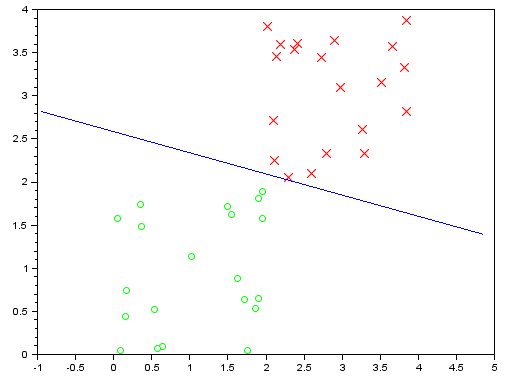
\includegraphics[width=0.75\textwidth]{perceptron.png}
 \caption{Wykres przedstawiający działanie perceptronu, dla \textit{alfa} = 0.5,\newline \textit{w} = [0.3374029 0.2356512 0.5928706]. \textit{k} (ilość iteracji) wyniosła 17.}
\end{figure}

\end{document}